\section{Dataset}
\label{sec:dataset}
For the task of bird species classification, many datasets are available online. 
However, these datasets encounter similar limitations for the research topic of this report. Most datasets focus on bird species that are not native to Europe.
Further, these datasets often provide a limited amount of data and are already heavily preselected. 
Therefore, a new dataset is created based on the comprehensive database of bird recordings available at \href{https://xeno-canto.org/}{xeno-canto.org} \cite{xeno-canto}. 
Xeno-canto is a website for sharing recordings of wildlife sounds, particularly bird songs. People from around the world can upload audio recordings to the website. The recordings 
are licensed under Creative Commons licenses and are free to use for non-commercial purposes.
To generate the dataset, the website's API is used to filter recordings and automatically download the files using the tool \textit{scikit-maad}~\cite{scikit-maad}.
For this project, recordings of common songbird species in Central Europe are searched for via the API. 
The recordings are required to have a length between $\num{5}$ and $\qty{300}{\second}$, as shorter recordings are not suitable for the approach used in this analysis, 
and longer recordings require more storage space. For this project, the recording type must include the tag \enquote{song} to filter for bird songs and exclude other bird sounds, 
such as woodpecker hammering.
Additionally, the sampling rate of the audio must be greater than $\qty{20000}{\hertz}$, and the audio must have sufficient overall quality 
(quality categories \enquote{A} and \enquote{B}). Often, other bird species can be heard in the background, which is problematic because this could lead to misclassifications between 
classes while training the classifier. Therefore, recordings that contain more than two other bird species in the background are removed.
Between $\num{100}$ and $\num{500}$ files are downloaded for each class. After applying all selection criteria, the dataset includes approximately $\num{17000}$ files across 
$\num{46}$ bird species classes, referenced by numerical \enquote{labels}, i.e., numbers from $\num{0}$ to $\num{45}$.
A list of the scientific and common names of the species corresponding to each label can be found in \Cref{sec:Appendix1}. 
The majority of the selected species are songbirds, but owl, swallow, and pigeon species are also included. In general, the audios can include background noise 
and calls of other species, as explained previously. The loudness, quality, and sampling rate vary significantly between recordings. 
Additionally, some recordings might include long segments with no bird sounds. All this increases the difficulty of the classification task but also enhances the robustness of 
a classifier trained on this data.
In \autoref{fig:example_data}, the waveforms and spectrograms for two recordings of different bird species are shown. The spectrograms highlight distinct features the CNN can learn 
to differentiate between these species.
\begin{figure}
    \centering
    \begin{subfigure}[c]{0.45\textwidth}
        \centering
        \includegraphics[width = .9\textwidth]{content/plots/wav_spec1.pdf}
        \subcaption{\enquote{Great Tit} (32) \cite{audio1}.}
    \end{subfigure}
    \begin{subfigure}[c]{0.45\textwidth}
        \centering
        \includegraphics[width = .9\textwidth]{content/plots/wav_spec2.pdf}
        \subcaption{\enquote{European Greenfinch} (29) \cite{audio2}.}
    \end{subfigure}
    \caption{Example spectrograms of audio recordings of different bird species.}
    \label{fig:example_data}
\end{figure} \\
To independently evaluate the classifier after hyperparameter optimization, a train-test split is performed, and $\qty{20}{\percent}$ of the data are set aside for exclusive use in the
final evaluation.
%shown in \autoref{fig:class_distributions}.
%\begin{figure}
%    \centering
%    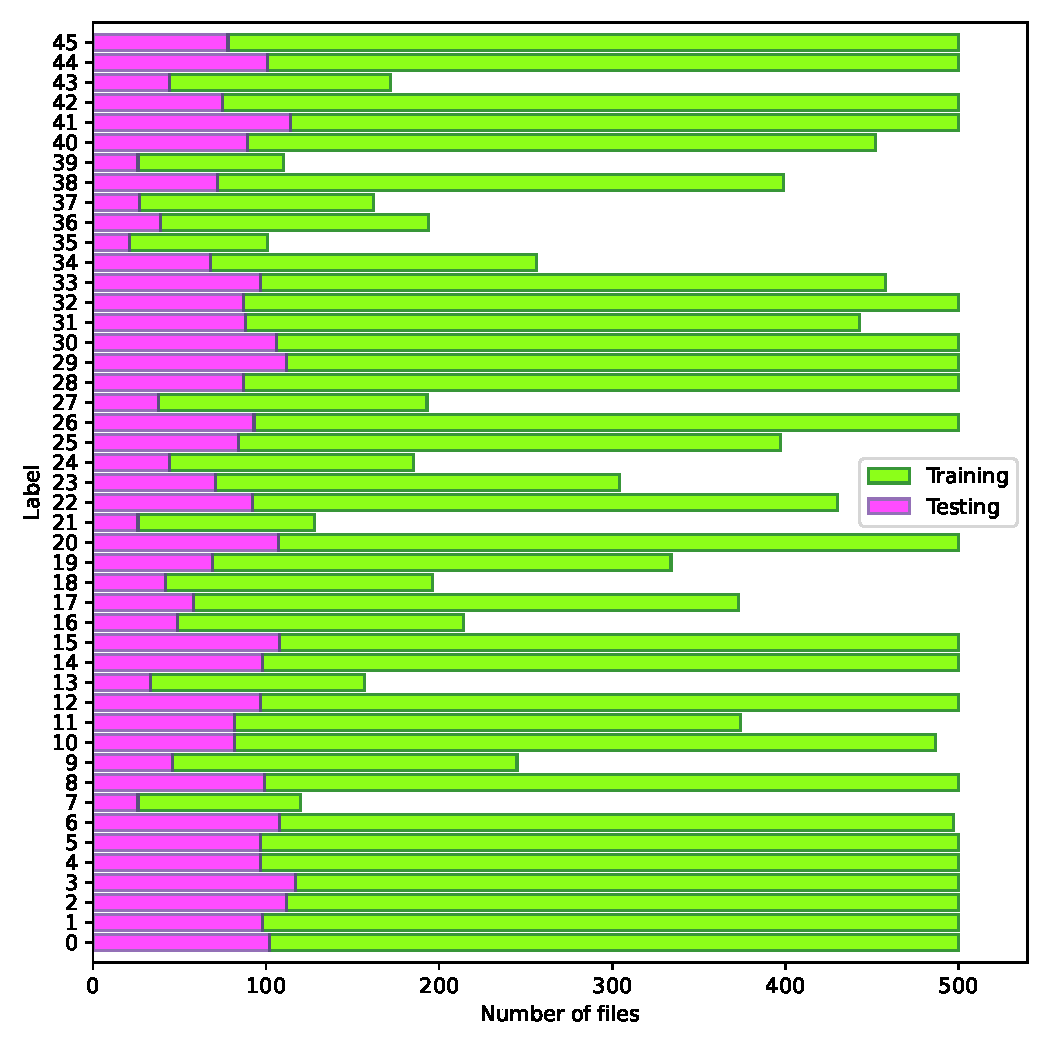
\includegraphics[width = .65\textwidth]{content/plots/class_distributions.pdf}
%    \caption{Class distributions of the training and test dataset.}
%    \label{fig:class_distributions}
%\end{figure}
%As can be seen from the plot, the classes are heavily imbalanced. 
The dataset's class distributions are strongly imbalanced.
Some classes have $\num{500}$ audio files, while others have only around $\num{100}$. 
This issue becomes more severe when considering the total audio length of the classes because classes with a lower number of available files often also have shorter audios. 
Plots showing the number of files and total audio length are presented in \Cref{sec:Appendix2}. To address this imbalance, classes with fewer files are upsampled to match the 
class with the highest number of files during training, and a balanced accuracy score is used in the evaluation.
\nopagebreak[4]
% - many prebuild dataset availabl
% - but: not for species in this region, limited amount of data, strongly preselected
% - introduce xeno canto: database for hobby bird enthusiasts
% - build own dataset
% - starting from 100 species
% - list and motivate requirements on recordings
% - describe final dataset
% - recordings have background noise, different quality, sampling rates
% - more than 1 bird might be heard
% - train test split
% - show examples for different species
% - show class (im)balances

